\hypertarget{TinyProtocol_8h}{}\section{src/\+Tiny\+Protocol.h File Reference}
\label{TinyProtocol_8h}\index{src/\+Tiny\+Protocol.\+h@{src/\+Tiny\+Protocol.\+h}}


Tiny protocol Arduino A\+PI.  


{\ttfamily \#include \char`\"{}Tiny\+Packet.\+h\char`\"{}}\newline
{\ttfamily \#include \char`\"{}Tiny\+Light\+Protocol.\+h\char`\"{}}\newline
{\ttfamily \#include \char`\"{}Tiny\+Protocol\+Hd.\+h\char`\"{}}\newline
{\ttfamily \#include \char`\"{}Tiny\+Protocol\+Fd.\+h\char`\"{}}\newline
Include dependency graph for Tiny\+Protocol.\+h\+:\nopagebreak
\begin{figure}[H]
\begin{center}
\leavevmode
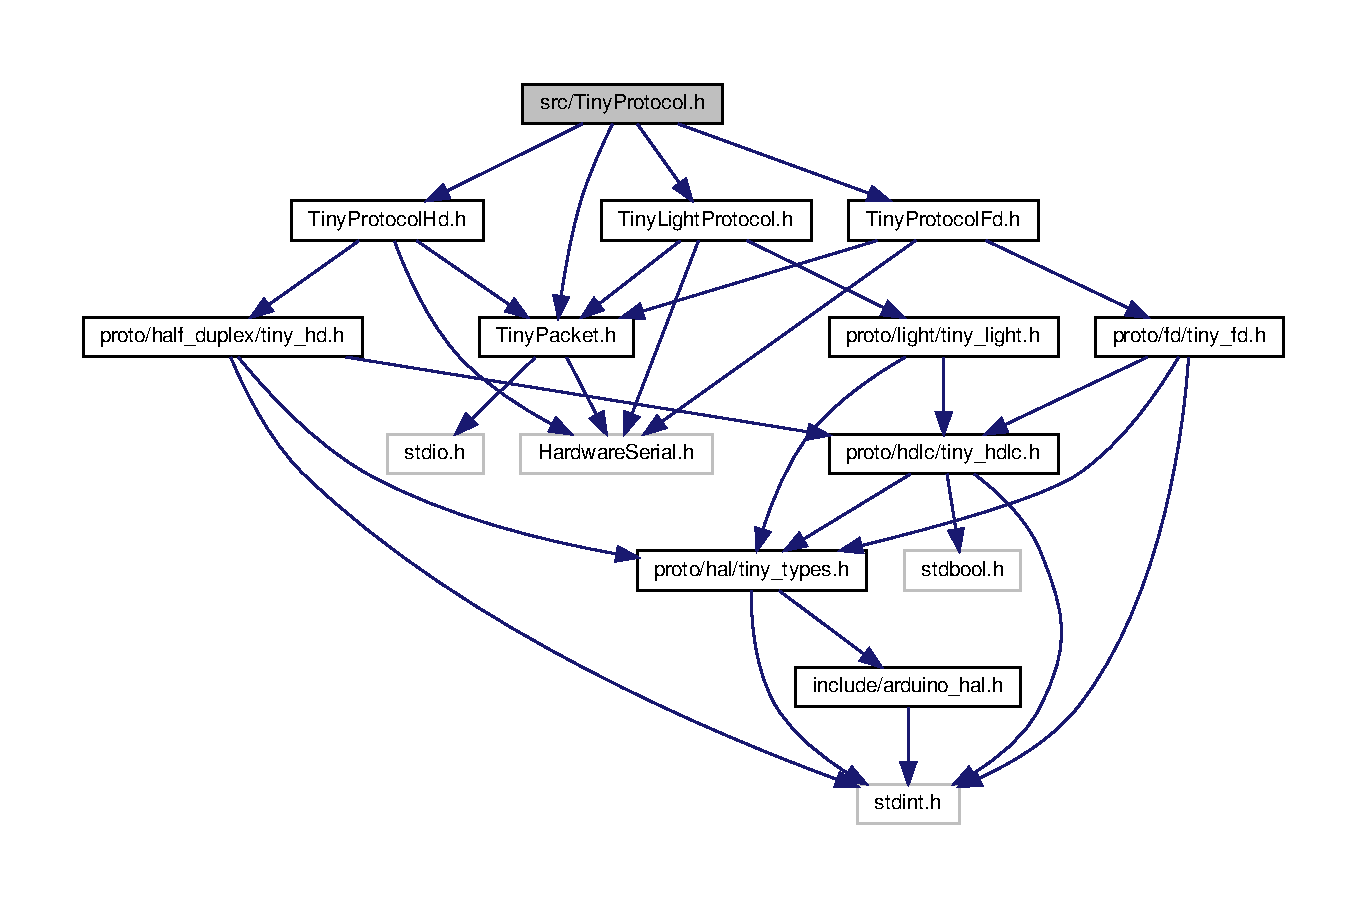
\includegraphics[width=350pt]{TinyProtocol_8h__incl}
\end{center}
\end{figure}


\subsection{Detailed Description}
Tiny protocol Arduino A\+PI. 

This is Tiny protocol implementation for microcontrollers 